\chapter{L'air, un mélange de gaz}\label{ch:g4:air-a-mixture-of-gases}

Un jour de vent, un cerf-volant tire sur sa ficelle et, sur le lac, une
voile se gonfle et pousse un bateau. Quelque chose les pousse, et
pourtant on ne voit rien. Ce quelque chose, c'est l'\omterm{def:g4:air-a-mixture-of-gases:air}{air}. On ne le voit
pas, mais il est partout autour de nous~: il remplit chaque bouteille
vide et chaque pièce, et nous en prenons à chaque respiration. De quoi
l'\omterm{def:g4:air-a-mixture-of-gases:air}{air} est-il fait~?

\begin{recall}
\omterm{def:g2:mixing-and-dissolving:mix}{Mélanger}, c'est mettre des choses différentes ensemble~; on obtient un
\omterm{def:g2:mixing-and-dissolving:mix}{mélange} de ces choses, et rien ne se perd quand on les \omterm{def:g2:mixing-and-dissolving:mix}{mélange}
(\cref{ch:g2:mixing-and-dissolving}).
\end{recall}

\begin{omfigure}
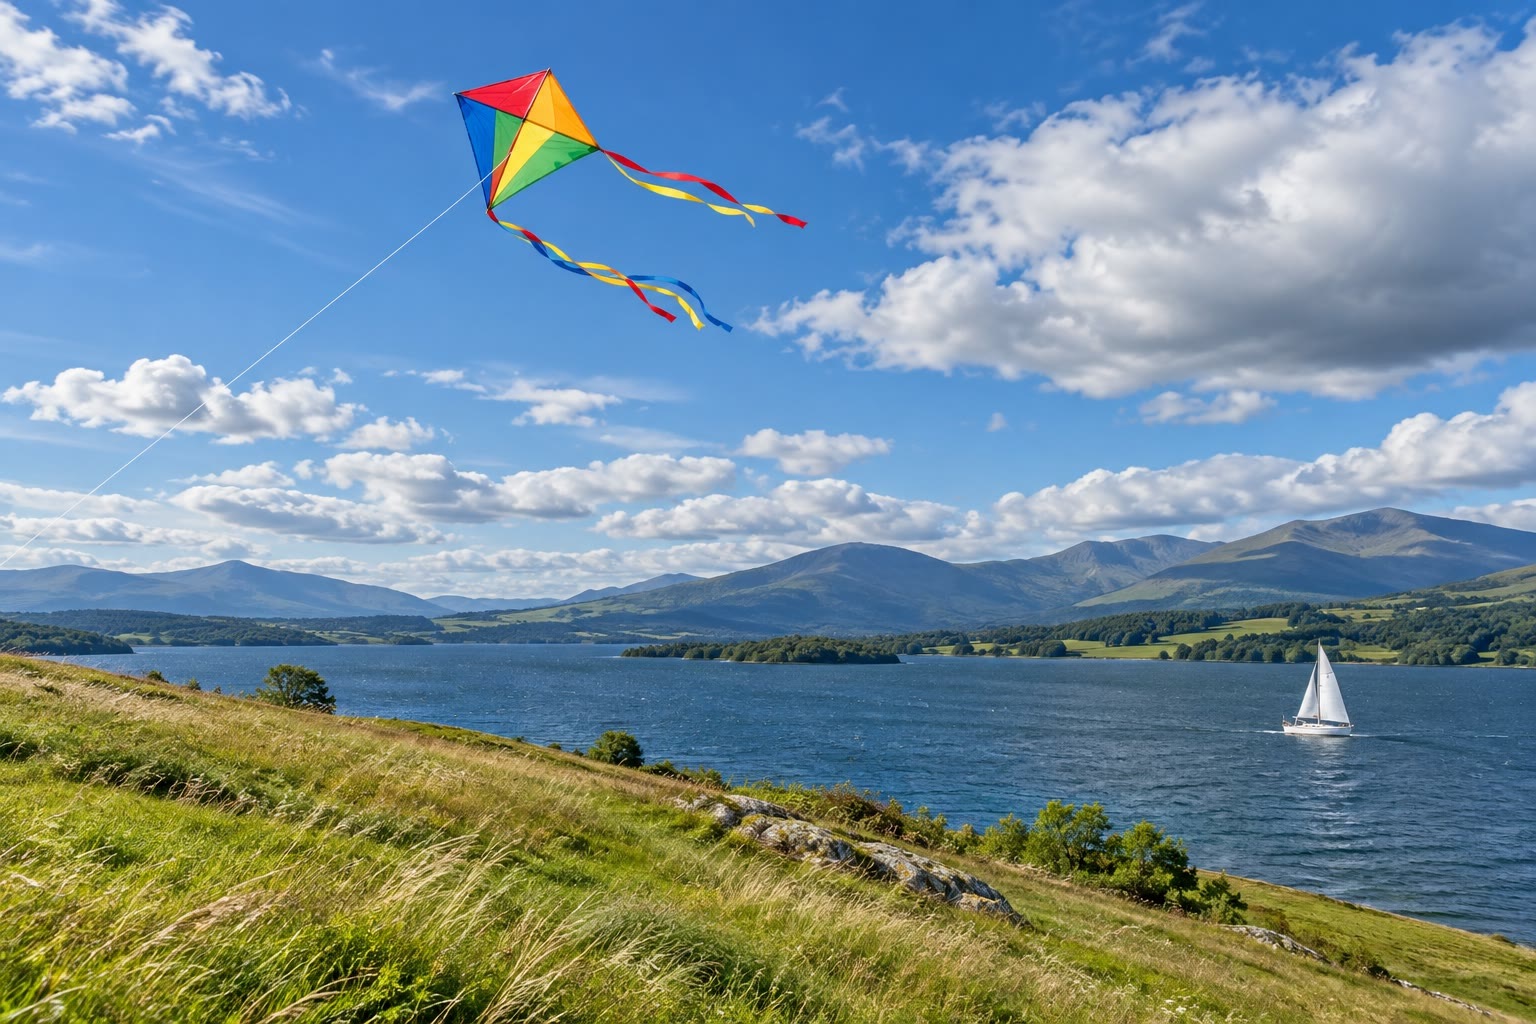
\includegraphics[width=0.6\linewidth]{images/book1/ai/g4-kite-day.jpg}

{\small Un cerf-volant et une voile~: l'\omterm{def:g4:air-a-mixture-of-gases:air}{air} ne se voit pas, mais il pousse.}
\end{omfigure}

\section{L'air est partout autour de nous}

\begin{example}[Un verre retourné]\label{ex:g4:air-a-mixture-of-gases:glass}
On enfonce un mouchoir en papier sec au fond d'un verre vide. On
retourne le verre et on l'enfonce bien droit dans une bassine d'eau.
Quand on le ressort, le mouchoir est toujours sec. Le verre n'était pas
vide~: il était plein d'\omterm{def:g4:air-a-mixture-of-gases:air}{air}, et l'\omterm{def:g4:air-a-mixture-of-gases:air}{air} a empêché l'eau d'entrer.
\end{example}

\begin{omfigure}
\begin{tikzpicture}[font=\small, scale=1.3]
  \pic[transform shape] at (0,0) {trough};
  % the upturned glass, rim at y = 0.35, base at y = 2.35
  \fill[white] (-0.8,0.5) rectangle (0.8,0.95);
  \pic[transform shape, rotate=180] at (0,2.35) {beaker={0}{white}};
  % the tissue at the top, inside
  \fill[white, draw=black!45, rounded corners=1.5pt] (-0.4,2.33) -- (-0.3,2.05)
    -- (-0.1,2.12) -- (0.05,1.98) -- (0.25,2.1) -- (0.42,2.02) -- (0.45,2.33) -- cycle;
  \draw[<-, omProp, thick] (0.45,2.12) -- (2.4,2.5) node[right, text=black]
    {un mouchoir sec};
  \draw[<-, omProp, thick] (0.3,1.2) -- (2.4,1.4) node[right, text=black]
    {de l'air~: il empêche l'eau d'entrer};
  \draw[<-, omProp, thick] (1.4,0.7) -- (2.4,0.55) node[right, text=black]
    {de l'eau};
\end{tikzpicture}

{\small On enfonce le verre retourné dans l'eau. L'\omterm{def:g4:air-a-mixture-of-gases:air}{air} emprisonné à
l'intérieur empêche l'eau d'entrer, et le mouchoir reste sec.}
\end{omfigure}


\begin{remark}[L'air est un gaz]\label{rem:g4:air-a-mixture-of-gases:gas}
L'\omterm{def:g4:air-a-mixture-of-gases:air}{air} est un gaz~: il n'a pas de forme propre et s'étale pour remplir
tout récipient. C'est pourtant de la matière, et un ballon plein d'\omterm{def:g4:air-a-mixture-of-gases:air}{air}
pèse un peu plus que le même ballon vide. Ce que sont les gaz, et
pourquoi ils se comportent ainsi, c'est le livre de physique qui le
raconte.
\end{remark}

\section{L'air est un mélange}

\begin{definition}[Air]\label{def:g4:air-a-mixture-of-gases:air}
L'\emph{air}\index{air} est le \omterm{def:g2:mixing-and-dissolving:mix}{mélange} de gaz qui entoure la Terre. Ce
n'est pas un gaz unique~: plusieurs gaz y sont mélangés, et on peut les
séparer les uns des autres.
\end{definition}

\begin{proposition}[De quoi l'air est fait]\label{prop:g4:air-a-mixture-of-gases:composition}
% ledger: air:N2, air:O2, air:Ar, air:trace, air:CO2, air:H2O
Si l'on met de côté sa vapeur d'eau, l'\omterm{def:g4:air-a-mixture-of-gases:air}{air} est fait~:
\begin{itemize}
  \item d'\textbf{azote}, environ les quatre cinquièmes de l'\omterm{def:g4:air-a-mixture-of-gases:air}{air}~;
  \item d'\textbf{oxygène}, environ un cinquième de l'\omterm{def:g4:air-a-mixture-of-gases:air}{air}~;
  \item d'un peu d'\textbf{argon}, environ 1 part sur 100~;
  \item d'un tout petit peu de \textbf{dioxyde de carbone}, environ 4
        parts sur 10\,000, et de minuscules quantités d'autres gaz.
\end{itemize}
L'\omterm{def:g4:air-a-mixture-of-gases:air}{air} contient aussi de la \textbf{vapeur d'eau}, invisible~: très peu
par une journée froide et sèche, jusqu'à environ 4 parts sur 100 par une
journée chaude et humide.
\end{proposition}

\begin{example}[Cent bouteilles d'air]\label{ex:g4:air-a-mixture-of-gases:hundred}
% ledger: air:N2, air:O2, air:Ar
Imagine 100 bouteilles d'\omterm{def:g4:air-a-mixture-of-gases:air}{air} sec, et les gaz de l'\omterm{def:g4:air-a-mixture-of-gases:air}{air} triés dans des
bouteilles séparées. Environ 78 bouteilles contiendraient de l'azote,
21 bouteilles de l'oxygène, et la dernière de l'argon, avec l'équivalent
de quelques gouttes de dioxyde de carbone et d'autres gaz.
\end{example}

\begin{omfigure}
\begin{tikzpicture}[font=\small, x=0.42cm, y=0.42cm]
  \foreach \k in {0,...,99} {
    \pgfmathtruncatemacro\col{mod(\k,10)}
    \pgfmathtruncatemacro\row{9-int(\k/10)}
    \ifnum\k<78 \def\c{omDef!45}\else\ifnum\k<99 \def\c{red!45}\else\def\c{cyan!60}\fi\fi
    \fill[\c, draw=white, line width=0.8pt] (\col,\row) rectangle ++(1,1);
  }
  \fill[omDef!45] (12,8) rectangle ++(1,1);
  \node[anchor=west] at (13.3,8.5) {azote~: 78 cases};
  \fill[red!45] (12,6) rectangle ++(1,1);
  \node[anchor=west] at (13.3,6.5) {oxygène~: 21 cases};
  \fill[cyan!60] (12,4) rectangle ++(1,1);
  \node[anchor=west, align=left] at (13.3,4.5) {argon, dioxyde de carbone\\ et le reste~: 1 case};
\end{tikzpicture}

{\small Cent cases d'\omterm{def:g4:air-a-mixture-of-gases:air}{air} sec. La case en bas à droite contient l'argon,
et le dioxyde de carbone, trop peu abondant pour être dessiné seul.}
\end{omfigure}

\begin{remark}[Des noms de gaz]\label{rem:g4:air-a-mixture-of-gases:names}
Azote, oxygène, argon et dioxyde de carbone sont des noms de gaz. Ils
sont tous incolores et n'ont pas d'odeur. Un chapitre suivant montre de
quoi chacun d'eux est fait, jusqu'aux toutes petites particules qui
forment toute la matière.
\end{remark}

\section{L'air que nous inspirons et expirons}

\begin{proposition}[L'air expiré]\label{prop:g4:air-a-mixture-of-gases:breath}
% ledger: breath:O2, breath:CO2, breath:N2, air:O2, air:CO2
L'\omterm{def:g4:air-a-mixture-of-gases:air}{air} que nous expirons n'est pas l'\omterm{def:g4:air-a-mixture-of-gases:air}{air} que nous avons inspiré. Notre
corps prend une partie de l'oxygène et rejette du dioxyde de carbone et
de la vapeur d'eau~:
\begin{itemize}
  \item environ 21 parts sur 100 de l'\omterm{def:g4:air-a-mixture-of-gases:air}{air} inspiré sont de l'oxygène,
        mais seulement environ 16 parts sur 100 de l'\omterm{def:g4:air-a-mixture-of-gases:air}{air} expiré~;
  \item le dioxyde de carbone passe d'environ 4 parts sur 10\,000 à
        environ 4 parts sur 100~: environ cent fois plus~;
  \item l'azote est expiré tel qu'il a été inspiré.
\end{itemize}
\end{proposition}

\begin{omfigure}
\begin{tikzpicture}
\begin{axis}[ybar, width=0.8\linewidth, height=5.2cm, bar width=12pt,
    ymin=0, ymax=90, ylabel={parts sur 100},
    symbolic x coords={nitrogen, oxygen, carbon dioxide}, xtick=data,
    xticklabels={azote, oxygène, dioxyde de carbone},
    tick label style={font=\small}, label style={font=\small},
    xticklabel style={text height=1.6ex, text depth=0.4ex},
    legend style={font=\small, at={(0.98,0.95)}, anchor=north east},
    nodes near coords, nodes near coords style={font=\footnotesize},
    enlarge x limits=0.25, axis lines*=left, ymajorgrids,
    grid style={gray!20}]
% ledger: air:N2, air:O2, air:CO2, breath:N2, breath:O2, breath:CO2 (rounded)
\addplot[fill=omDef!45, draw=omDef] coordinates
  {(nitrogen,78) (oxygen,21) (carbon dioxide,0)};
\addplot[fill=omProp!55, draw=omProp] coordinates
  {(nitrogen,78) (oxygen,16) (carbon dioxide,4)};
\legend{air inspiré, air expiré}
\end{axis}
\end{tikzpicture}

{\small L'\omterm{def:g4:air-a-mixture-of-gases:air}{air} inspiré et l'\omterm{def:g4:air-a-mixture-of-gases:air}{air} expiré, en parts sur 100 (vapeur d'eau
mise à part, nombres arrondis). Le dioxyde de carbone de l'\omterm{def:g4:air-a-mixture-of-gases:air}{air} inspiré,
4 parts sur 10\,000, est trop peu abondant pour apparaître sous forme de
barre.}
\end{omfigure}

\begin{example}[Une salle pleine de monde]\label{ex:g4:air-a-mixture-of-gases:room}
Dans une petite salle de classe aux fenêtres fermées, trente personnes
rejettent du dioxyde de carbone toute la matinée. Peu à peu, l'\omterm{def:g4:air-a-mixture-of-gases:air}{air} de la
salle contient moins d'oxygène et plus de dioxyde de carbone, et chacun
se sent fatigué. Ouvrir les fenêtres fait entrer de l'\omterm{def:g4:air-a-mixture-of-gases:air}{air} frais.
\end{example}

\begin{omfigure}
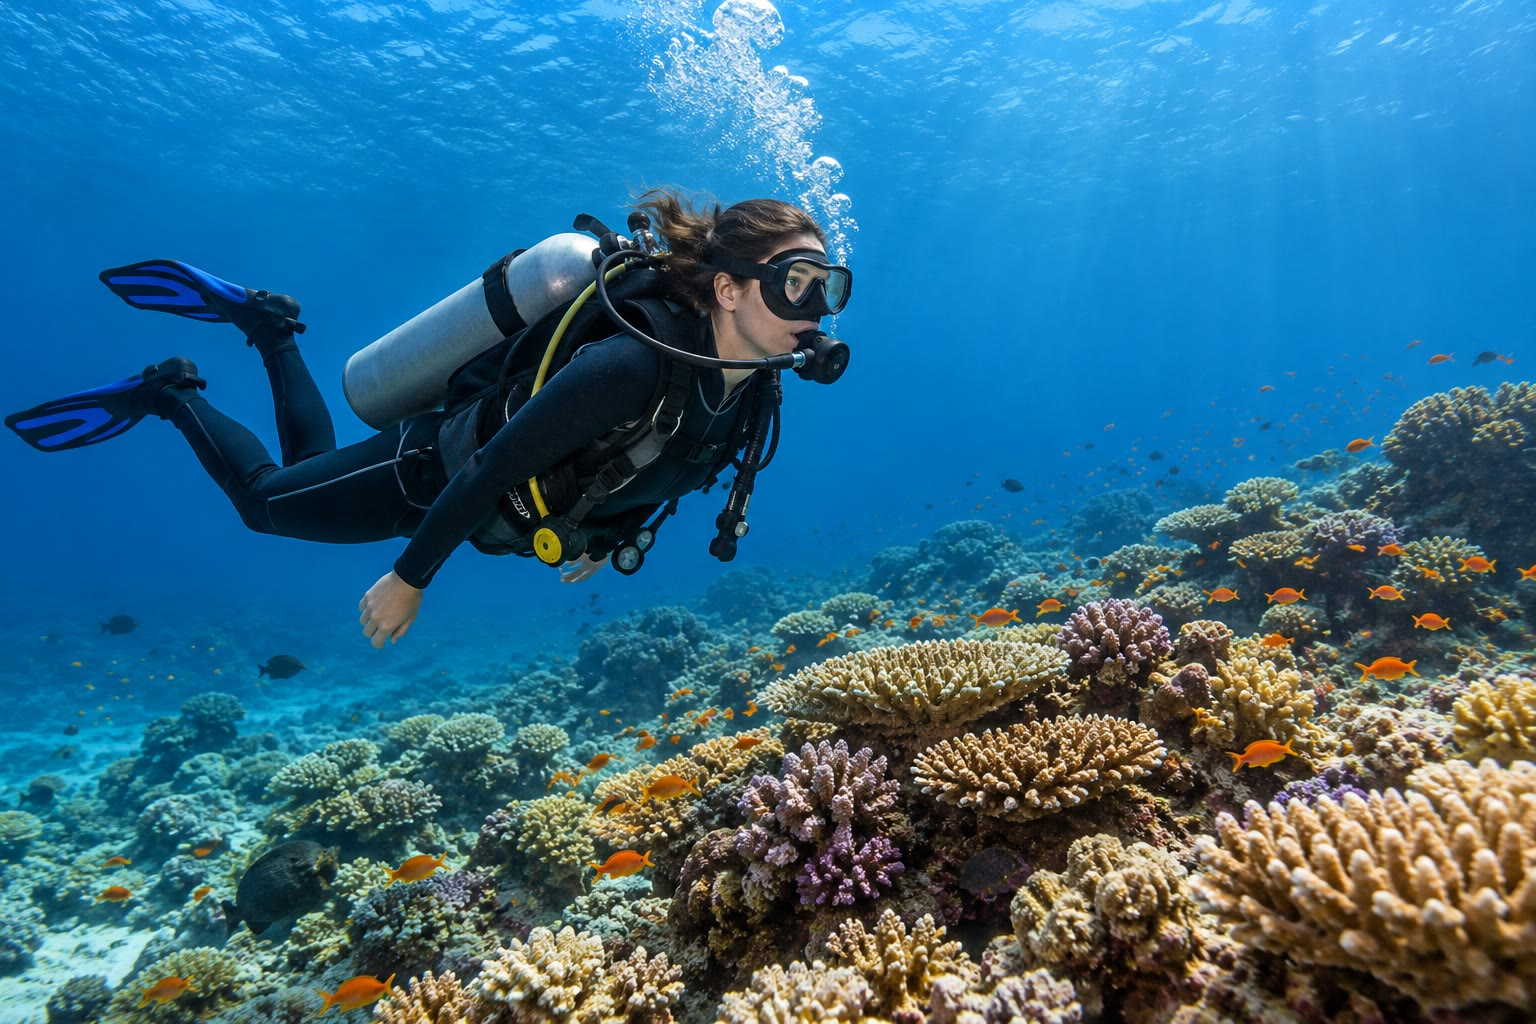
\includegraphics[width=0.55\linewidth]{images/book1/ai/g4-scuba-diver.jpg}

{\small Un plongeur respire l'\omterm{def:g4:air-a-mixture-of-gases:air}{air} de la bouteille qu'il porte sur le
dos~; les bulles sont l'\omterm{def:g4:air-a-mixture-of-gases:air}{air} qu'il expire.}
\end{omfigure}

\begin{remark}[Pourquoi les plongeurs respirent de l'air]\label{rem:g4:air-a-mixture-of-gases:diver}
La bouteille d'un plongeur est remplie d'\omterm{def:g4:air-a-mixture-of-gases:air}{air} comprimé dans un petit
volume, pas d'oxygène pur~: respirer de l'oxygène pur en profondeur est
dangereux. L'azote de l'\omterm{def:g4:air-a-mixture-of-gases:air}{air} est là pour diluer l'oxygène.
\end{remark}

\section{De l'oxygène pour la vie et pour le feu}

\begin{proposition}[L'oxygène est consommé par les êtres vivants et par les flammes]\label{prop:g4:air-a-mixture-of-gases:oxygen}
De tous les gaz de l'\omterm{def:g4:air-a-mixture-of-gases:air}{air}, l'oxygène est celui dont ont besoin les êtres
vivants et les flammes. Les animaux et les humains le prélèvent en
respirant~; une flamme le prend dans l'\omterm{def:g4:air-a-mixture-of-gases:air}{air} qui l'entoure. Les plantes
vertes, à la lumière du jour, rendent de l'oxygène à l'\omterm{def:g4:air-a-mixture-of-gases:air}{air}.
\end{proposition}

\begin{inthelab}[Une bougie sous un bocal]
L'enseignant allume une bougie posée sur un carreau et descend lentement
un grand bocal en verre par-dessus. La flamme rapetisse, vacille et
s'éteint au bout de quelques secondes~: autour de la flamme, l'\omterm{def:g4:air-a-mixture-of-gases:air}{air}
contient trop peu d'oxygène pour qu'elle continue de brûler. Sous un
bocal deux fois plus grand, la bougie brûle environ deux fois plus
longtemps, car il y a environ deux fois plus d'\omterm{def:g4:air-a-mixture-of-gases:air}{air}, donc deux fois plus
d'oxygène, à consommer.
\end{inthelab}

\begin{omfigure}
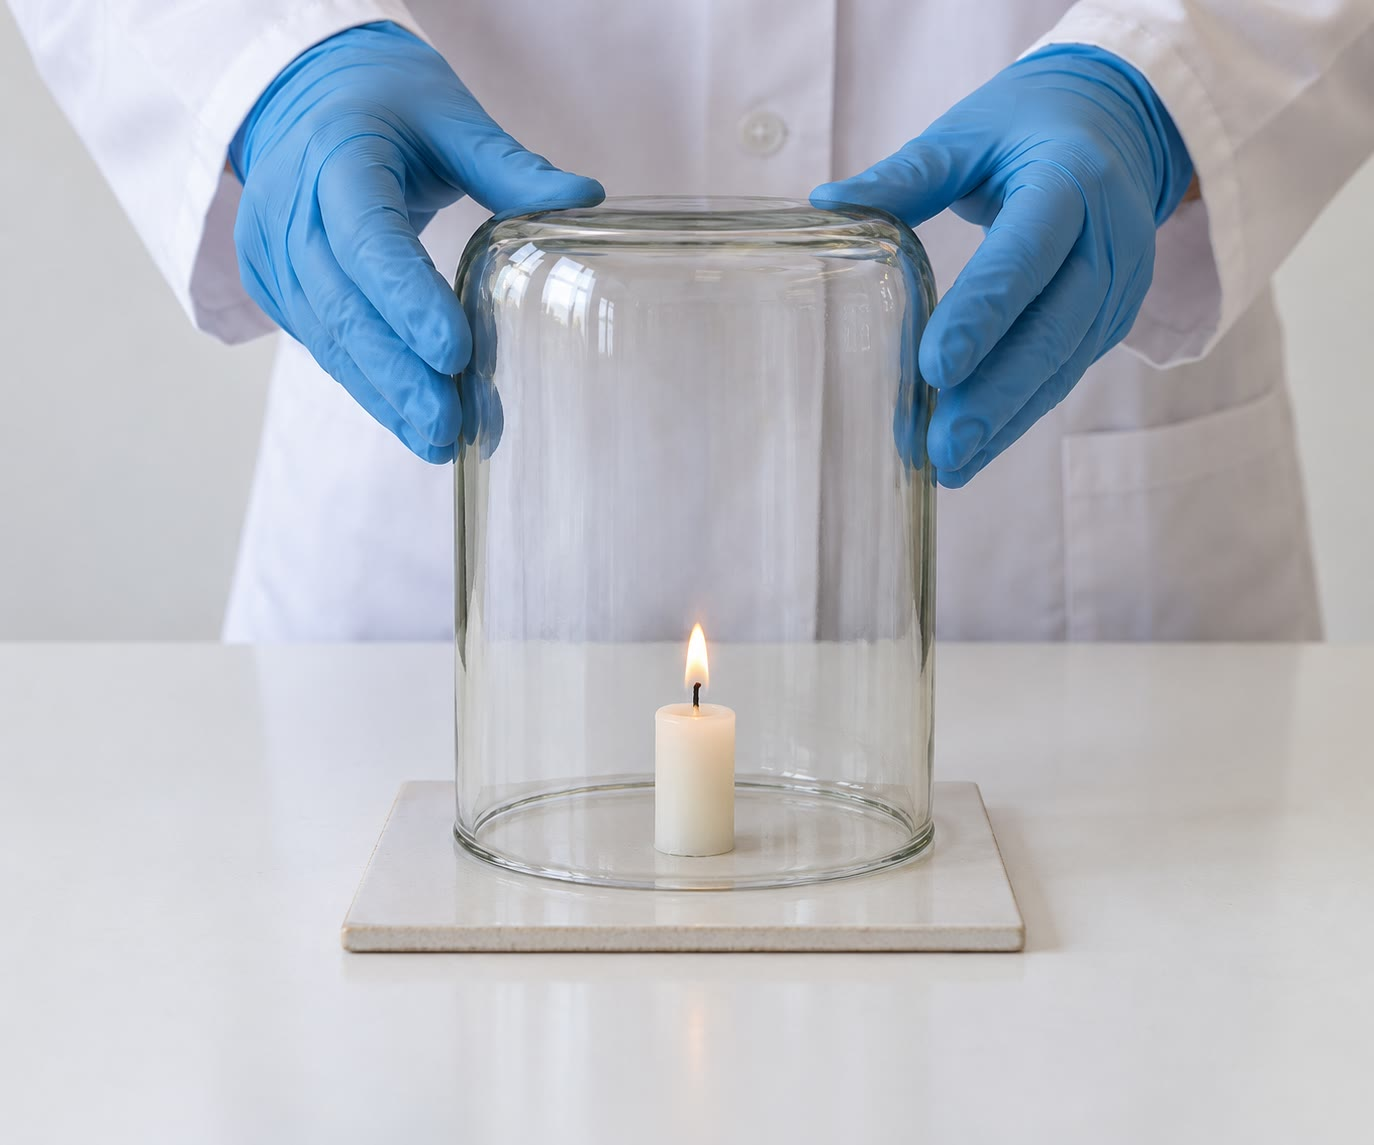
\includegraphics[width=0.5\linewidth]{images/book1/ai/g4-candle-jar-lab.jpg}

{\small Une bougie sous un bocal en verre s'éteint quand il ne reste plus
assez d'oxygène autour de sa flamme.}
\end{omfigure}

\begin{remark}[L'azote ne brûle pas]\label{rem:g4:air-a-mixture-of-gases:nitrogen}
L'azote est la plus grande partie de l'\omterm{def:g4:air-a-mixture-of-gases:air}{air}, et pourtant il n'entretient
pas une flamme, et notre corps ne l'utilise pas. Si l'\omterm{def:g4:air-a-mixture-of-gases:air}{air} n'était que de
l'azote, nous ne pourrions pas respirer et rien ne pourrait brûler.
\end{remark}

\section{Exercices}

\begin{exercise}[$\star$]\label{exo:g4:air-a-mixture-of-gases:1}
L'\omterm{def:g4:air-a-mixture-of-gases:air}{air} est-il un gaz unique ou un \omterm{def:g2:mixing-and-dissolving:mix}{mélange}~? Nomme les deux principaux gaz
de l'\omterm{def:g4:air-a-mixture-of-gases:air}{air}.
\end{exercise}

\begin{exercise}[$\star$]\label{exo:g4:air-a-mixture-of-gases:2}
Quelle fraction de l'\omterm{def:g4:air-a-mixture-of-gases:air}{air}, environ, est de l'azote~? Quelle fraction,
environ, est de l'oxygène~?
\end{exercise}

\begin{exercise}[$\star$]\label{exo:g4:air-a-mixture-of-gases:3}
Dans 100 litres d'\omterm{def:g4:air-a-mixture-of-gases:air}{air} sec, combien de litres, environ, sont de
l'azote~? Combien de litres, environ, sont de l'oxygène~?
\end{exercise}

\begin{exercise}[$\star$]\label{exo:g4:air-a-mixture-of-gases:4}
On enfonce une bouteille vide, retournée, dans une bassine d'eau.
Pourquoi l'eau ne remplit-elle pas la bouteille~?
\end{exercise}

\begin{exercise}[$\star$]\label{exo:g4:air-a-mixture-of-gases:5}
Regarde le diagramme en barres. De quel gaz y a-t-il moins dans l'\omterm{def:g4:air-a-mixture-of-gases:air}{air}
expiré~? De quel gaz y a-t-il plus~?
\end{exercise}

\begin{exercise}[$\star$]\label{exo:g4:air-a-mixture-of-gases:6}
De quel gaz de l'\omterm{def:g4:air-a-mixture-of-gases:air}{air} une flamme a-t-elle besoin~? De quel gaz de l'\omterm{def:g4:air-a-mixture-of-gases:air}{air}
avons-nous besoin pour respirer~?
\end{exercise}

\begin{exercise}[$\star$]\label{exo:g4:air-a-mixture-of-gases:7}
Regarde la figure aux 100 cases. Combien de cases sont de l'azote~?
Combien n'en sont pas~?
\end{exercise}

\begin{exercise}[$\star$]\label{exo:g4:air-a-mixture-of-gases:8}
Pourquoi une bougie placée sous un bocal s'éteint-elle au bout d'un
moment~?
\end{exercise}

\begin{exercise}[$\star$]\label{exo:g4:air-a-mixture-of-gases:9}
Dans 500 litres d'\omterm{def:g4:air-a-mixture-of-gases:air}{air}, combien de litres, environ, sont de l'oxygène~?
(Un cinquième de l'\omterm{def:g4:air-a-mixture-of-gases:air}{air} est de l'oxygène.)
\end{exercise}

\begin{exercise}[$\star\star$]\label{exo:g4:air-a-mixture-of-gases:10}
Pourquoi est-il bon d'ouvrir les fenêtres d'une salle de classe entre
les cours~?
\end{exercise}

\begin{exercise}[$\star\star$]\label{exo:g4:air-a-mixture-of-gases:11}
Une bougie brûle pendant 10 secondes sous un petit bocal. Combien de
temps, environ, brûlerait-elle sous un bocal contenant trois fois plus
d'\omterm{def:g4:air-a-mixture-of-gases:air}{air}~?
\end{exercise}
